\documentclass[a4paper,10pt]{article}
\usepackage[left=1.5cm, right=1.5cm, top=2cm, bottom=2cm]{geometry}
\usepackage{xcolor}
\usepackage{titlesec}
\usepackage{graphicx} % Pour inclure des images
\usepackage{fontawesome}
\usepackage{hyperref}
\usepackage{enumitem}

% Couleurs personnalisées
\definecolor{maincolor}{RGB}{41, 128, 185}
\definecolor{textcolor}{RGB}{44, 62, 80}
\definecolor{accentcolor}{RGB}{231, 76, 60}
\definecolor{bgcolor}{RGB}{255, 255, 255}


\begin{document}

\pagecolor{bgcolor} % Application de la couleur de fond
\pagestyle{empty}

% En-tête
\begin{center}
    % Ajouter l'image de votre photo ici
    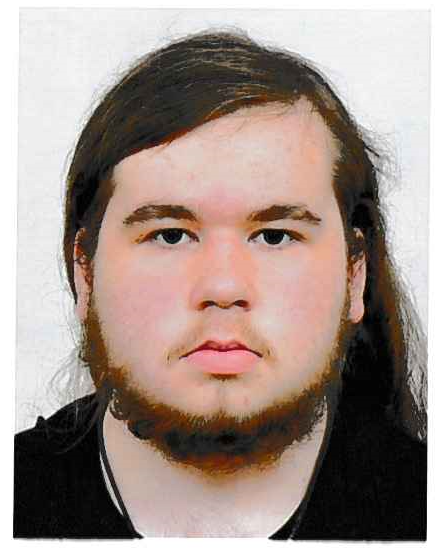
\includegraphics[width=0.2\textwidth]{cvpp.png} \\
    \vspace{3mm}
    {\Huge \textbf{HALL Eliott}}\\
    \vspace{5mm}
    \faEnvelope~\href{mailto:eliott.hall.pro@gmail.com}{eliott.hall.pro@gmail.com} \quad
    \faPhone~+33 6 34 48 62 33 \quad
    \faGithub~\href{https://github.com/malkiium}{github.com/malkiium}
\end{center}

\vspace{5mm}

% Formation
\section{Formation}
\textbf{Lycée Général Schumann-Perret} \hfill {2022}\\
{\color{accentcolor}Baccalauréat Général --- Maths-SVT}

\vspace{3mm}
\textbf{Université du Havre --- Biologie} \hfill {2023 --- 2024}\\
{\color{accentcolor}L1}

\vspace{3mm}
\textbf{Université du Havre --- Informatique} \hfill {2024 --- 2025}\\
{\color{accentcolor}L1}

\vspace{5mm}

% Compétences
\section{Compétences}
\begin{itemize}[label=\textbullet, font=\color{maincolor}\large]
    \item \textbf{Langages:} Python, Java, HTML, CSS, C, C++, LaTeX
    \item \textbf{Outils:} Git, Linux, Excel, Word, PowerPoint, Visual Studio Code, Visual Studio, IntelliJ IDEA, PyCharm, WebStorm
\end{itemize}

\vspace{5mm}

% Langues
\section{Langues}
\begin{tabular}{ll}
    \textbf{Français:} & Langue maternelle \\
    \textbf{Anglais:} & Langue maternelle
\end{tabular}

%intérêts
\section{Intérêts}
\begin{itemize}[label=\textbullet, font=\color{maincolor}\large]
    \item Informatique
    \item sciences
    \item Musique
    \item Jeux vidéo
    \item Photographie
    \item Video montage
\end{itemize}

\end{document}

